\chapter{问题描述与背景知识}
\label{cha:problem}
本章将首先对论文的攻击模型,论文需要解决的问题和论文预计达到的目标进行定义,然后对论文中需要用到的背景知识进行介绍。

\section{问题定义}
在本节中,我们将正式定义方案的攻击模型,方案需要解决的问题以及方案需要实现的目标。

\subsection{攻击模型}
在单用户场景中,数据持有者和数据搜索用户是同一人,而在多用户场景中,这两者是分开的。我们假定数据持有者本身和数据搜索用户是可信的,而不可信,而提供存储和搜索服务的云服务器是不可信的,即 1) 云服务器会试图从用户的加密数据和搜索请求中推断出一些隐私信息; 2) 云服务器有可能会因为外部攻击、配置错误、软件错误等原因背离原有协议,从而导致产生数据新鲜性攻击和数据完整性攻击,用以节省其自身的计算开销和通信开销。数据新鲜性攻击和数据完整性攻击的正式定义如下:

\begin{definition}[\textbf{数据新鲜性攻击}]\label{def:freshness}
    {\itshape
			在对称加密搜索中,数据新鲜性攻击是指一个恶意的云服务器试图从旧数据集中返回搜索结果,而不从最新的数据集中返回搜索结果。正式地,让$\Delta_{n-1} = \{\delta_1,\delta_2,\cdots,\delta_{n-1}\}$ 代表用户数据集的历史版本, $\delta_n$ 代表用户的最新数据集,云服务器返回的搜索结果为 $\delta_i$ 的子集,其中 $1 \le i \le n-1$。
      %A data freshness attack in SSE is that a malicious server (or an attacker) attempts to return the historical version of the search result, not the most recently updated version. Formally, let $\Delta_{n-1} = \{\delta_1,\delta_2,\cdots,\delta_{n-1}\}$ denote the historical version of the dataset and $\delta_n$ is the latest version. However, the search result returned by the server is retrieved from $\delta_i$ where $1 \le i \le n-1$.
    }
\end{definition}

\begin{definition}[\textbf{数据完整性攻击}]\label{def:integrity}
    {\itshape
			在对称加密搜索中,数据完整性攻击是指一个恶意的云服务器试图篡改搜索结果,阻止数据搜索用户获取到完整的搜索结果。正式地,让 $\tau$ 代表对称加密搜索方案中的搜索令牌,$\delta_i$ 代表数据集,其中 $1 \le i \le n$。对应的搜索结果应为 $\mathcal{F}(\delta_i, \tau)$,但云服务器返回的搜索结果为 $\mathcal{G}(\delta_i, \tau)$, 其中$\mathcal{G}(\delta_i, \tau) \neq \mathcal{F}(\delta_i, \tau)$。
      %A data integrity attack in SSE is that a malicious server (or an attacker) attempts to tamper with the search result to prevent authenticated users from accessing the complete and correct search result. Formally, let $\tau$ be the search token of the SSE scheme, and $\delta_i$ be the dataset, where $1 \le i \le n$, the corresponding search result should be $\mathcal{F}(\delta_i, \tau)$, but the result returned by the server is $\mathcal{G}(\delta_i, \tau)$, where $\mathcal{G}(\delta_i, \tau) \neq \mathcal{F}(\delta_i, \tau)$.
    }
\end{definition}

%We assume that the data owner is trusted and the data users authorized by the data owner are also trusted\footnote{Please refer to Section \ref{Sec:Discussion} for details on how we can enforce such assumption in practice with multi-user access control techniques.}.
%We consider cloud services performing searchable symmetric encryption (SSE) to be untrusted, which means 1) cloud services intends to derive some sensitive information from the encrypted data and the queries; 2) cloud services may deviate from the prescribed protocols and mount a data freshness attack or a data integrity attack to save its computation or communication cost. The definitions of the data freshness attack and the data integrity attack are presented as follow:

%在可验证加密搜索中,由于服务器不诚信导致的安全性攻击主要可以分为以下两种:
%	重放攻击(Replay Attack):在加密搜索中,重放攻击是指服务器(攻击者)试图返回旧的搜索结果,而不是最新的搜索结果。我们用Δ_n={δ_1,δ_2,⋯,δ_n}来表示旧版本的数据集,用δ_(n+1)来表示最新的数据集,则服务器返回的搜索结果是数据集δ_i的搜索结果,其中1≤i≤n。
%	数据完整性攻击(Data Integrity Attack):在加密搜索中,数据完整性攻击是指服务器(攻击者)试图不让用户获取完整的搜索结果。我们用τ来表示加密搜索中用户的搜索陷门,用户应该得到的搜索结果为F(τ),而服务器返回的搜索结果为G(τ),其中G(τ)⊂F(τ)并且G(τ)可能为∅。
%重放攻击仅存在于动态的加密搜索方案中,在数据库静态的情况下不存在。但现实中,动态数据库较为常见,因此重放攻击是可验证加密搜索必须要解决的问题。数据完整性攻击不仅包括服务器少返回搜索结果的情况还包括了服务器不返回搜索结果来规避结果验证的情况。


\subsection{设计目标}

本论文旨在设计一种通用的可验证加密搜索方案,即该方案可以和任意加密搜索方案相结合,甚至包括公钥加密搜索方案,使其能够完成结果验证的功能。本方案将现有的加密搜索方案当做黑盒,总体来说,需要满足以下几个需求:

\begin{enumerate}
	\item \textbf{机密性:} 数据和关键字的机密性是加密搜索最基本的安全需求。它保证了用户的明文数据和关键字信息无法被其他不可信第三方所得到。并且保证了敌手无法从方案的加密数据集,验证索引以及搜索关键字中推断出任何有用的隐私信息。
	%The confidentiality of data and keywords is the most important privacy requirements in SSE. It ensures that users' plaintext data and keywords cannot be revealed by any unauthorized parties, and an adversary cannot learn any useful information about files and keywords through the proof index and update tokens used in %\name.
	%In our scheme, data privacy and keyword privacy is guaranteed by its underlying cipher. Moreover, the search pattern of our scheme is hiding by trading the space.
	\item \textbf{可验证性:} 一个可验证的对称加密搜索方案应该能够验证搜索结果的正确性和完整性,即防止数据新鲜性攻击和数据完整性攻击。%A verifiable SSE scheme should be able to verify the freshness and integrity of the search results for users.
	%In our scheme, we design a proof algorithm based on the proof structure to detect the dara integrity attacks and meanwhile use the chained-timestamp mechanism to detect the replay attacks.
	\item \textbf{高效性:} 一个可验证对称加密搜索方案应该达到次线性的计算复杂度,即对数复杂度 $O(log(|W|))$,其中 $|W|$ 是关键字的总数,并且应该在支持用户数据更新的情况下仍然能达到该复杂度。注意,这里的计算复杂度仅仅指服务器提供结果验证服务时所需的额外计算复杂度,不包括加密搜索方案本身带来的计算复杂度。%A verifiable SSE scheme should achieve sublinear computational complexity, e.g. logarithmic $O(log(|W|))$, where $|W|$ is the number of keywords, even with file update. Note that, the computational complexity only refers to the cost of searching operations for verification, which does not include the complexity of the searching operations in the existing SSE schemes.
	%Update efficiency, search efficiency and verification efficiency is the most improtant indicator we aim to achieve. In our scheme, we leverage the Mekle Patricia Tree (MPT) which provides the $O(log(n))$ efficiency for search and update which is the optimal solution to the best of our knowledge.
\end{enumerate}

	%机密性:数据和关键字机密性是加密搜索中最重要的隐私需求。其中,数据机密性要求用户的明文数据不能被云服务器获取,关键字机密性要求关键字和文件的相关性不能被云服务器所推断。
	%可验证性:一个可验证的加密搜索方案应该能够验证搜索结果的正确性和完整性,即防止重放攻击和数据完整性攻击。
	%效率:一个可验证的加密搜索方案应该在搜索和更新时具有合理的计算复杂度,例如O(log⁡(|W|)),其中|W|是关键字的数目。


  %This paper aims to provide result verification for any SSE schemes, including but not limited to~\cite{stefanov2014practical,cash2014dynamic,kamara2012dynamic}. Therefore, we treat an existing SSE scheme as a black box such that our proposed scheme can be applied to these SSE schemes for result verification.

\section{背景知识}

\subsection{增量哈希}
增量哈希 (Incremental Hash, IH) 由Bellare等人提出~\cite{bellare1994incremental},并被已有的加密搜索方案~\cite{kamara2011cs2}所使用。增量哈希函数是一个抗碰撞的函数:$IH: \{0,1\}^* \rightarrow \{0,1\}^l$,两个随机字符串通过增量哈希函数相加或相减后,生成的哈希值不会产生碰撞。举例来说,假设 $D_w$ 是一个包含关键字 $w$ 的数据集合,它的增量哈希值为 $H$。 当一个新数据 $d$ 加入到 $D_w$ 中后, 新的数据集合变为 $D_w'$ ,即 $D_w+d$。对于原有数据集 $D_w$ 来说,数据 $d$ 的加入只是微小的变动。增量哈希函数可以基于数据 $d$ 和现有哈希值 $H$,并通过“加法”操作快速的计算出新文件集 $D_w'$ 的一个抗碰撞哈希值,而不需要基于新文件集 $D_w'$ 重新计算哈希值,这使得哈希操作的性能得到了较大的提升。
 %Incremental hash was proposed by Bellare et al.~\cite{bellare1994incremental} and was used by existing SSE schemes, e.g., CS2~\cite{kamara2011cs2}. An incremental hash function is a collision-resistant function $IH: \{0,1\}^* \rightarrow \{0,1\}^l$, with which the addition or the subtraction operation of two random strings on the $IH$ does not produce a collision. For example, assuming $F$ is a file collection that contains the keyword $k$. After a new file $f$ is inserted to $F$, the file collection becomes $F'$ (i.e., $F+f$), which means the new file $f$ is a slight change according to $F$.  Therefore, an incremental hash function can be used to quickly compute the corresponding collision-resist hash value after a file change. More detailed descriptions can be found in~\cite{kamara2011cs2}.


%【IH】Thank the reviewer for pointing out this issue. We reviewed the incremental hash in Section 2. An incremental hash function is a collision-resistant function, which was first proposed by Bellare et al. [22]. We revised the description of the incremental hash in Section 2.
%In our scheme, if a file collection of a data owner is changed, the data owner uses the incremental hash function to quickly calculate a collision-resistance hash value of the changed data, which achieves high efficiency in computing hash values. Another advantage is that, when a file is added or deleted, a collision-resistance hash value ensures the security of our scheme during update.
\subsection{默克尔帕特里夏树}
默克尔帕特里夏树,即MPT,最早在以太坊~ \cite{wood2014ethereum, merklepatriciatree} (Ethereum) 中提出,它将传统的字典树 (Trie Tree) 和默克尔树结合,使得该树同时具有查找和验证的功能。MPT具有三种类型的节点,分别为叶子节点(Leaf Node,LN),分支节点(Branch Node,BN)和扩展节点(Extension Node,EN)。其中叶子节点存储了键值对,扩展节点也存储了键值对,但扩展节点的“键值”分别为其子节点的公共前缀和子节点的哈希值。分支节点有17个元素,其中前16个元素代表了该节点上有可能的分支,即16个十六进制数字,第17个元素为值。当某一个“键”在该分支节点匹配完成时,该“键”对应的“值”就存储该元素中。

\begin{figure}[t]
\centering
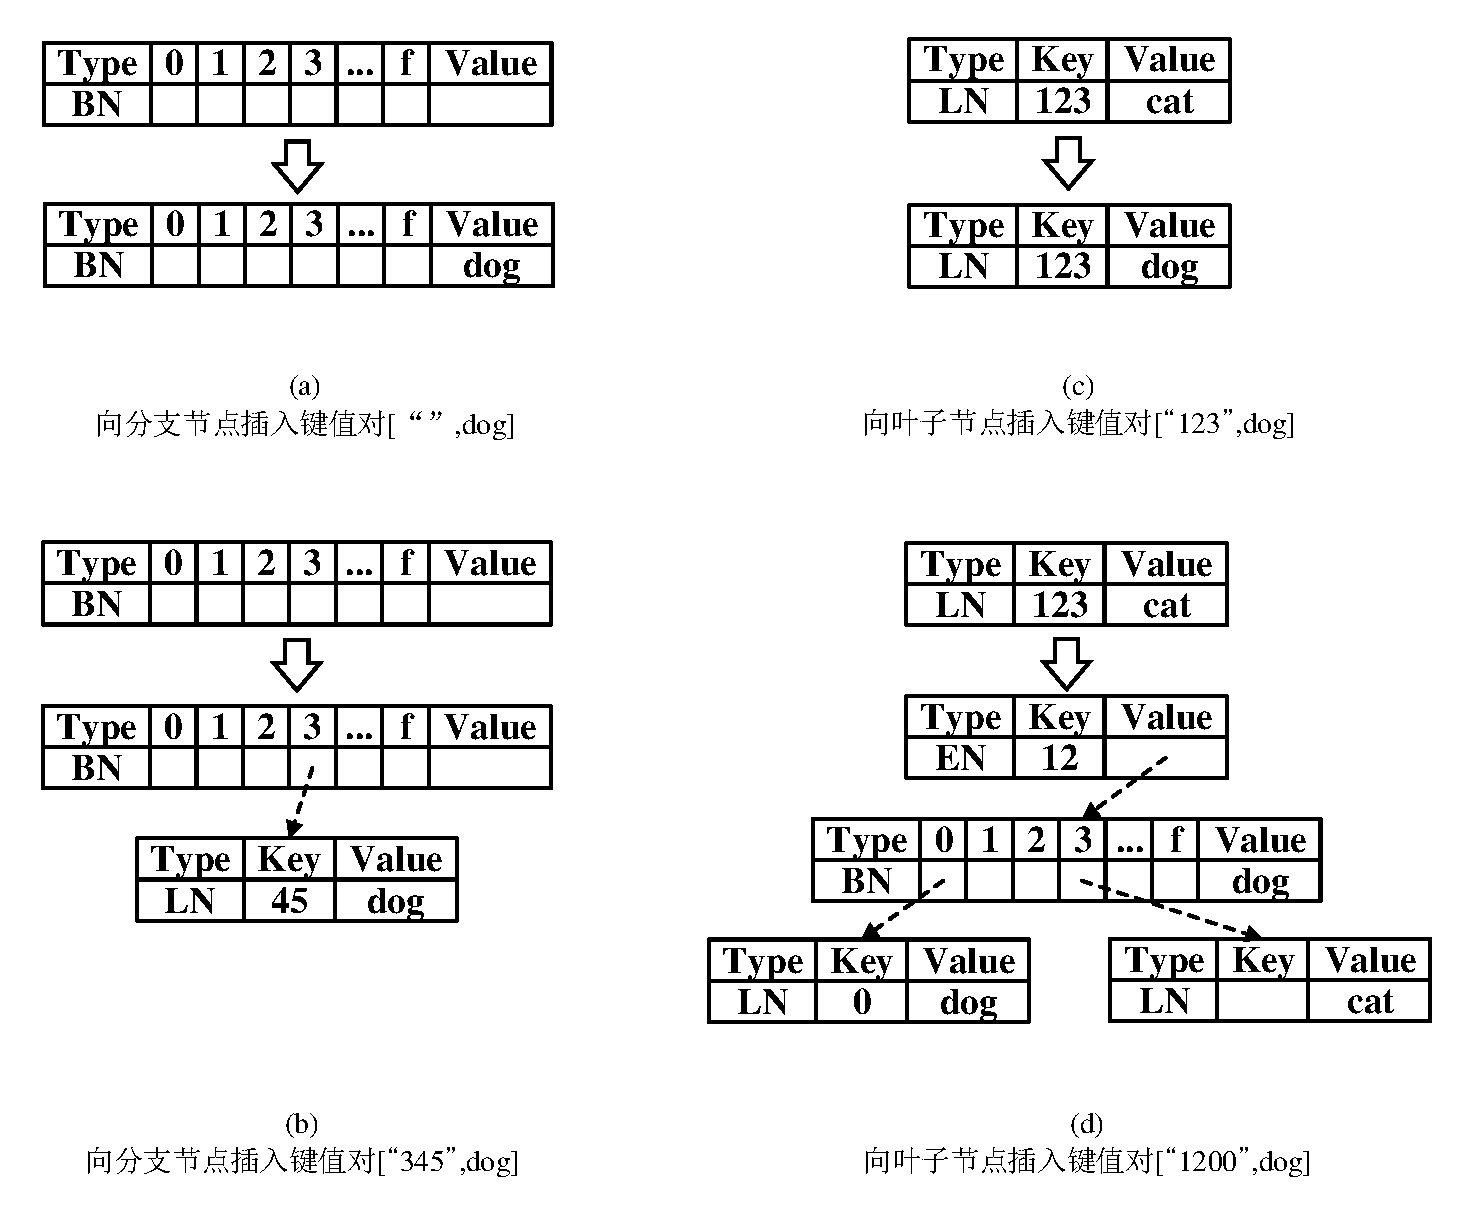
\includegraphics[width=6 in]{fig/MPTUpdate}
\DeclareGraphicsExtensions.
\caption{MPT的更新过程}
\label{fig:MPTUpdate}
\end{figure}

图~\ref{fig:MPTUpdate} 通过四个简单的例子展示了MPT的插入过程。首先是将一个“键值对”插入到分支节点的情况,有两种可能。如果当前的键空间已经为空,我们可以直接将“值”插入到分支节点的第17个位置,如图\ref{fig:MPTUpdate}(a)所示。否则,在经过了分支节点匹配后,键空间中“剩余键”和“值”将会存储在分支节点指向的一个新的叶子节点中,如图\ref{fig:MPTUpdate}(b)所示。其次是将“键值对”插入到叶子节点的情况,也有两种可能。如果当前键空间中“剩余键”与叶子节点中的“键”正好匹配,直接将叶子节点中的“值”修改为新的“值”即可,如图\ref{fig:MPTUpdate}(c)所示。否则,我们将找到当前键空间“剩余键”和叶子节点“键”的共同前缀,将其作为一个新建的扩展节点的“键”,并新建一个分支节点,指向该扩展节点。我们将匹配完扩展节点和分支节点后的“剩余键”作为一个新建叶子节点的键,并将原有的叶子节点和这个新建的叶子节点作为子节点插入到分支节点对应的元素空间中,如图\ref{fig:MPTUpdate}(d)所示。

注意,MPT中的每一个节点都通过可递归长度前缀法~\cite{RLPcode}(Recursive Length Prefix, RLP) 进行了编码并对编码值再进行了哈希。数据库中存储了每个节点的“键值对”,其中“键”为该节点RLP编码的哈希,“值”为该节点的RLP编码。这样每个节点可以通过他的哈希值被引用,同时保证了MPT的可搜索性和可验证性。通过这种方式,MPT的根哈希成为了整棵树的指纹信息,根哈希的值由所有下层节点的哈希值所决定,任何节点的微小改变都会导致根哈希的值发生变化。此外,MPT与默克尔树不同,MPT是完全确定性的,即一组相同的“键值对”采用不同的顺序插入到MPT中,最终得到的根节点哈希值是相同的,而默克尔树不具有这个性质。
%The Merkle Patricia Tree (MPT) is first proposed in Ethereum~ \cite{wood2014ethereum, merkle_patricia_tree}, which combines the Trie Tree and the Merkle Tree for data update efficiency. There are three kinds of nodes in an MPT to achieve the goal. Leaf Nodes(LN) represents [key,value] pairs. Extension Nodes(EN) represent [key,value] pairs where keys are the public prefixes and their values are the hashes of the next nodes. The Branch Nodes (BN) are used to store possible branches when the prefixes of the keywords differ, which is presented with 17 elements. Among the 17 elements, the first 16 elements represent the 16 possible hex characters in a key and the last element stores a value if a key in a [key,value] pair matches the node.

%Note that, each node of the MPT is represented by its hash and is encoded using Recursive Length Prefix (RLP) code that is mainly used to encode arbitrarily binary data~\cite{RLP_code}, which ensures the cryptographically security of the search operations. The root hash in MPT becomes a fingerprint of the entire tree and is computed based on all hashes of nodes below. Therefore, any modification in a node would incur recomputation of the root hash. Note that, the MPT is fully deterministic, meaning that an MPT with the same [key,value] pairs is exactly the same regardless of the order of insertion, which is different from the Merkle Tree.

\subsection{对称加密搜索}
云存储的出现使得用户可以在云端对数据进行备份,并且节省了用户本地存储的开销。因此越来越多的用户选择将他们的数据上传给云服务器。但由于云服务存在诸多安全风险,数据应该加密后再上传,但这使得用户失去了对其数据的搜索能力。一个简单的解决方案是,用户将密文数据全部下载下来以后,对其进行解密,然后在明文数据上进行搜索。但这种解决方案需要用户下载整个数据库,带来的通信开销和存储开销很大,在许多设备上势必是不可能实现的,例如移动设备由于流量和存储空间都有限,就不可能采用这种简单的方案。加密搜索的提出将这种搜索功能转移到了云端,并且同时不造成明文数据泄露。
目前,大部分的对称加密搜索方案都采用了建立一个加密索引$\gamma$的方式来解决此问题。该加密索引根据用户数据集$\mathcal{D}$来构建。用户首先需要从该数据集中提取出所有的关键字集合$\mathcal{W}$,并将$\mathcal{W}$中的每一个关键字$w_i$与包含该关键字的文件$D_w$相关联,其中$i \in \{1,\cdots, |W|\}$。最后用户通过加密每一个$(w_i, D_w)$对,建立搜索索引$\gamma$,而加密后的关键字$w_i$将会被用户用于后续搜索。一个对称加密搜索方案的常见框架如图~\ref{fig:SSE}所示。

\begin{figure}[h]
\centering
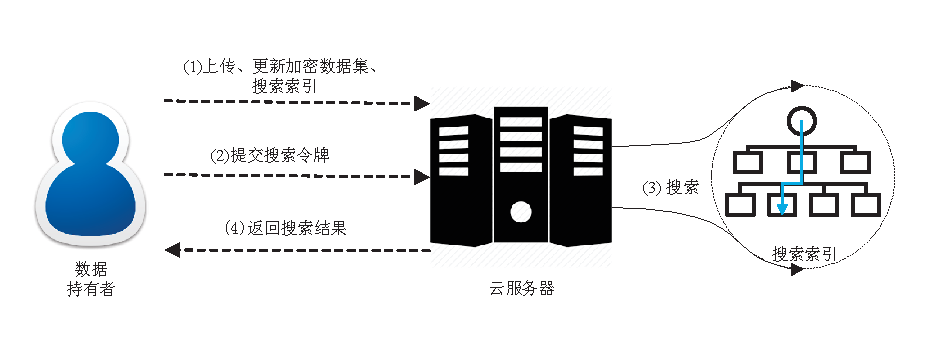
\includegraphics[width=6 in]{fig/SSE}
\DeclareGraphicsExtensions.
\caption{对称加密搜索方案的框架}
\label{fig:SSE}
\end{figure}

用户首先需要对自身持有的明文数据集进行加密并上传到云端,与此同时,用户还需要根据该数据集生成一个加密索引。该加密索引保证了云服务器可以在不解密加密索引和密文数据集的情况下,对用户的密文数据进行搜索。当用户需要搜索数据时,他将生成一个令牌,该令牌与搜索关键字相关,使得用户可以在不暴露关键字内容的情况下进行内容搜索。



\subsection{多用户对称加密搜索}

根据Bosch等人提出的综述~\cite{bosch2015survey},现有的加密搜索方案可以分为四种类别:单方写入/单方读取 (Single writer/Single reader, S/S), 单方写入/多方读取(Single writer/Multi-reader, S/M),多方写入/单方读取(Multi- writer/Single reader, M/S) 以及多方写入/多方读取(Multi-writer/Multi-reader, M/M)。在本文中我们主要针对单方写入/多方读取这种多用户场景,因为该场景多用于个人用户的存储与数据共享场景中,而多方写入/单方读取的场景多用于邮件数据存储,多方写入/多方读取场景主要用户企业级云存储方案中。

本文并不致力于研究一种访问控制方案来实现多用户的加密搜索方案,因为针对用户的访问控制问题目前已有许多研究,例如基于角色的访问控制策略( Role-based Access Control Policies)~\cite{sandhu1996role,ferraiolo2001proposed}等等细粒度的访问控制方案。数据持有者可以根据每个用户的不同职责来为其分配不同的访问权限,每个角色对应于一种访问权限,例如只读等等。本方案可以为实现了这种数据访问控制的多用户加密搜索方案提供结果验证功能。目前已有相关研究提出了这种支持单方写入/多方读取的多用户加密搜索方案~\cite{curtmola2011searchable, jarecki2013outsourced,sun2016efficient},例如广播加密方案(Broadcase Encryption, BE)和基于属性加密搜索方案(Attribute-Based Encryption, ABE)等等。

如图~\ref{fig:MSSE}所示,本文以广播加密方案~\cite{curtmola2011searchable}为例,阐述数据持有者如何对数据搜索用户进行访问控制。
\begin{figure}[h]
\centering
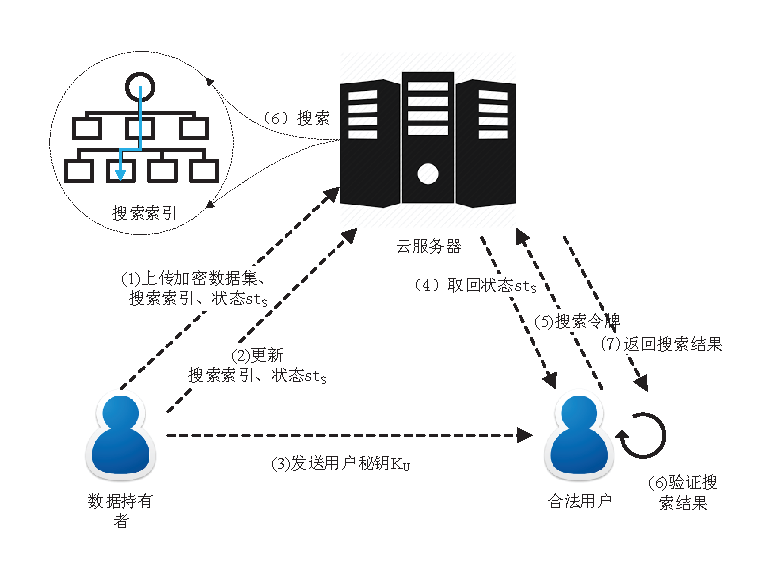
\includegraphics[width=6 in]{fig/MSSE}
\DeclareGraphicsExtensions.
\caption{多用户下的对称加密搜索方案的框架}
\label{fig:MSSE}
\end{figure}

数据持有者通过私钥$K_O$和用户身份信息生成用户私钥$K_U$,他将用户私钥$K_U$发送给该用户$U$,并将一个状态$st_S$更新给云服务器,其中$st_S$由数据持有者的合法用户群$G$和一个对称秘钥$r$计算得到。为了搜索一个关键字$w$, 用户需要从服务器上获取状态$st_S$,并通过用户私钥$K_U$解密出其中包含的对称秘钥$r$,随后用户通过计算$\Phi_r(\tau_w)$并上传给服务器来进行访问控制验证。云服务器在收到$\Phi_r(\tau_w)$,可以通过计算$\tau_w = \Phi_r^{-1}(\Phi_r(\tau_w))$提取出其中包含的搜索令牌$\tau_w$。
注意,如果数据持有者需要剔除一个用户$U$,他仅需要重新选择一个对称秘钥$r'$,然后根据新的用户群$G'= G \backslash U$重新生成一个状态$st^{'}_S$即可。只要云服务器和被剔除的用户不存在共谋,一个被剔除的用户不再属于用户群$G'$,因此他将无法从从状态$st^{'}_S$中解密出对称秘钥$r'$,因此也无法生成一个合法的搜索令牌。
通过这种广播加密方案,数据持有者可以方便的控制他的合法搜索用户,并且不需要再每次剔除一个用户时重新生成验证索引。
